\documentclass[12pt]{article}
\usepackage{amsmath}
\usepackage{amssymb}
\usepackage{geometry}
\usepackage{enumerate}
\usepackage{natbib}
\usepackage{float}%稳定图片位置
\usepackage{graphicx}%画图
\usepackage[english]{babel}
\usepackage{a4wide}
\usepackage{indentfirst}%缩进
\usepackage{enumerate}%加序号
\usepackage{multirow}%合并行
\title{\large UM-SJTU JOINT INSTITUTE\\Introduction to Computer Organization\\(VE370)\\\ \\\ \\\ \\\ \\\ \\\ \\\ \\\ \\\ \\\ \\\
Project1\\\ \\\ \\\ \\\ \\\ \\\ \\\ }
\author{Name: Pan Chongdan\\ID: 516370910121}
\date{Date: \today}

\begin{document}
\maketitle
\newpage
\section{Introduction}
The project asks me to develop a MIPS assembly program that operates on a data segment consisting of an array of 32-bit unsigned integers. In the text segment of memory, I'll write a procedure called main that implements the main() function and other subroutines described below. Assemble, simulate, and carefully comment the file. I'll also screen print my simulation results and explain the results by annotating the screen prints. I compose an array whose size 30. 
\begin{figure}[H]
\centering
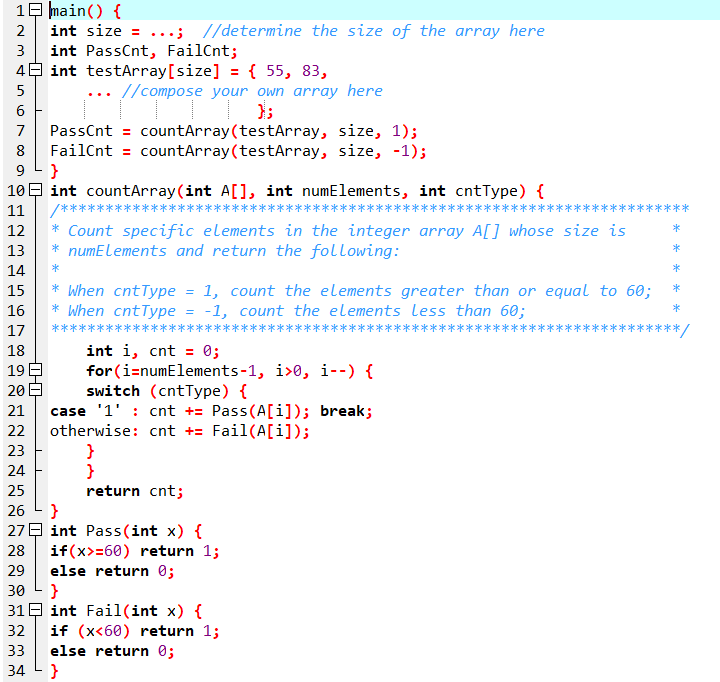
\includegraphics[scale=0.5]{cpp.png}
\caption{Original C++ code}
\end{figure}
The program will count the numbers of elements less than 60 or bigger than 60 in my array.
\section{Procedure}
\subsection{Generate the Array for simulation}
First, I write a CPP code to generate an array whose size is 30.
\begin{figure}[H]
\centering
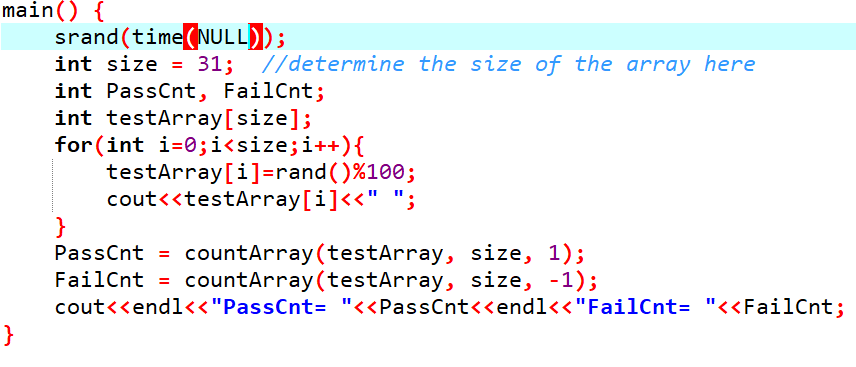
\includegraphics[scale=0.5]{cpp2.png}
\caption{C++ code to generate the array}
\end{figure}
For simulation, I choose the array with elements :
\par 55 84 13 48 29 75 53 42 97 2 81 36 19 69 55 0 55 94 68 1 62 76 41 66 9 10 12 28 65 62
\par where 12 passed and 18 failed
\section{Conclusion}
It takes me a long time to finish my project, and here is my simulation result and my conclusion.
\begin{figure}[H]
\centering
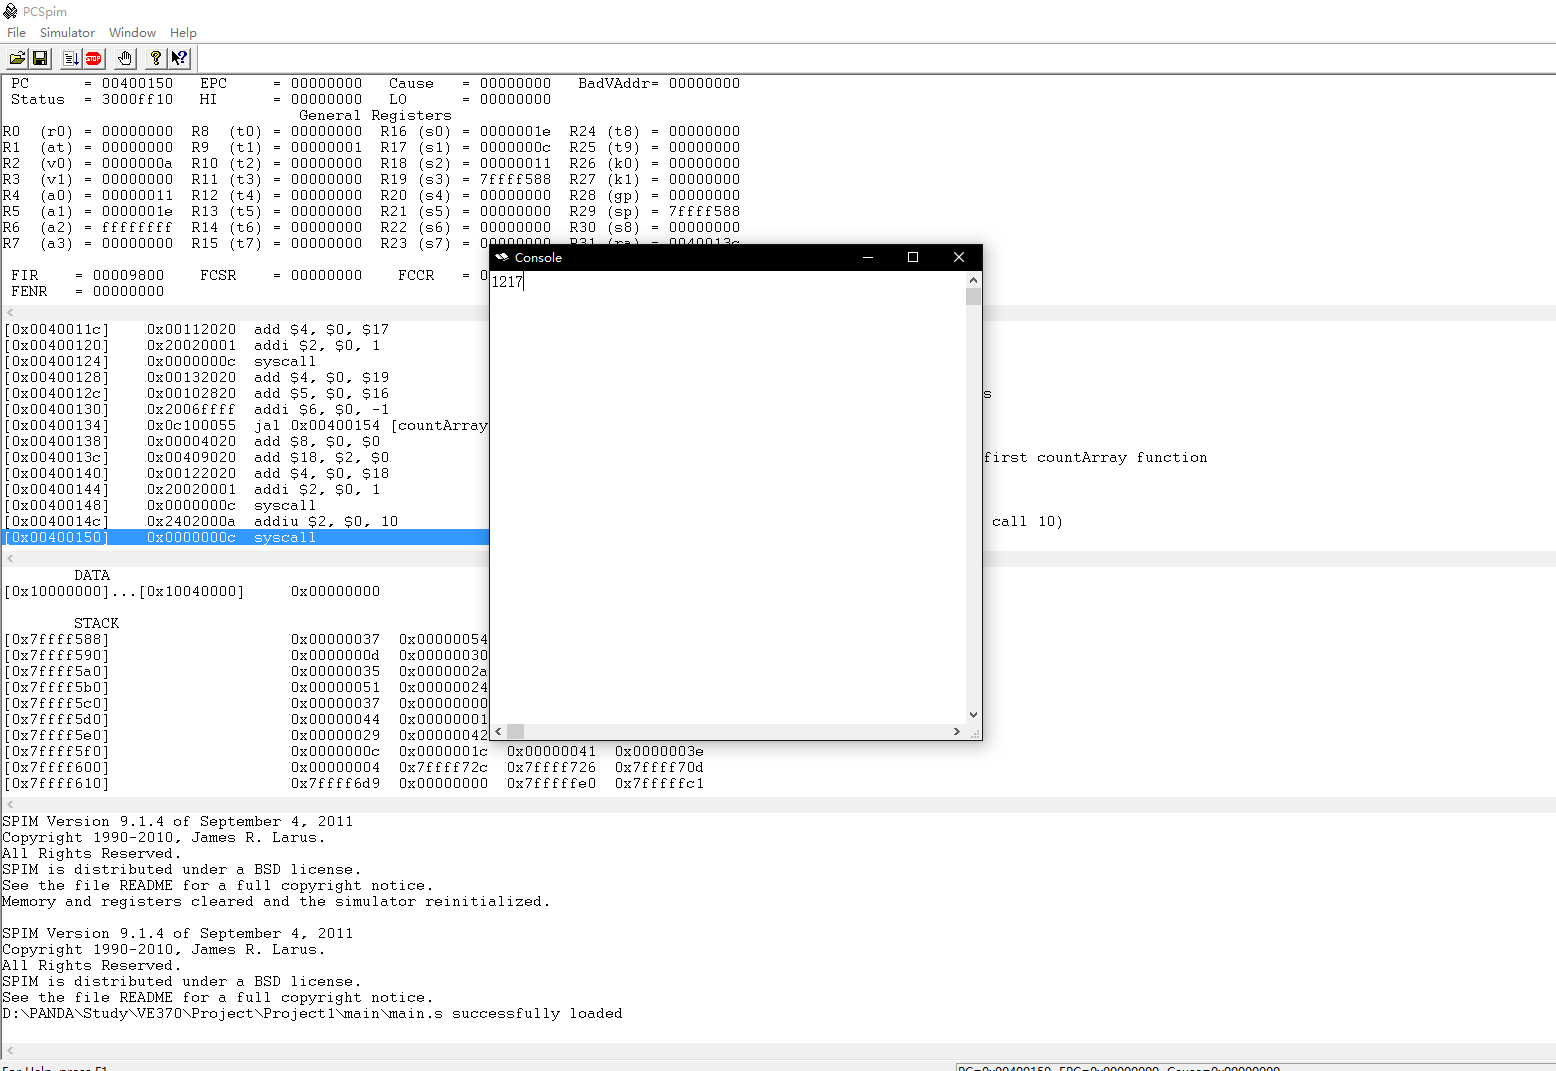
\includegraphics[scale=0.3]{PCSpim.png}
\end{figure}
\begin{enumerate}
\item From the console we can see the number for pass is 12 and for failure is 17, it;s obvious to see their sum is 29, which is smaller than the size. I think it's because in the statement of the for loop given from the project introduction, the i>0 should changed to i>=0 because we haven't visited element 0 yet. So we miss a element smaller than 60, which is 55 in my array.
\item Write meaningless code for delay is very important. At first, I can't run my code but I can't find where is the problem. Then, it took me a long time to debug through breakpoints, and in the end I found I need to place some delay code at the jr and jal instruction, otherwise mips will do another instruction and change the value in registers.
\item As you can see from my result, I can;t separate 12 from 17 because I don't know how to output a string. At first, I find some way on the internet by using la and .asciiz code, but it doesn't work afterwards. I think it's because the setting of PCSpim and we'll learn some other way later.
\end{enumerate}
\section{Appendix}
\begin{figure}[H]
\centering
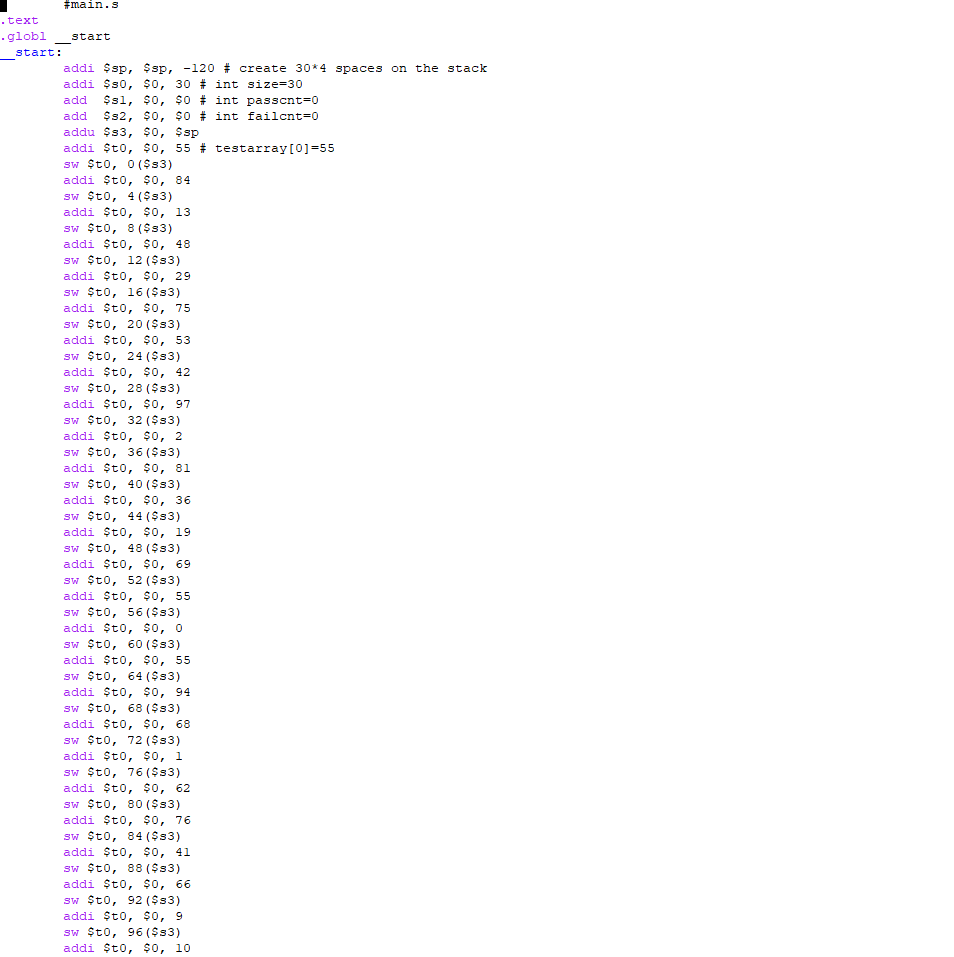
\includegraphics[scale=0.6]{mips1.png}
\end{figure}
\begin{figure}[H]
\centering
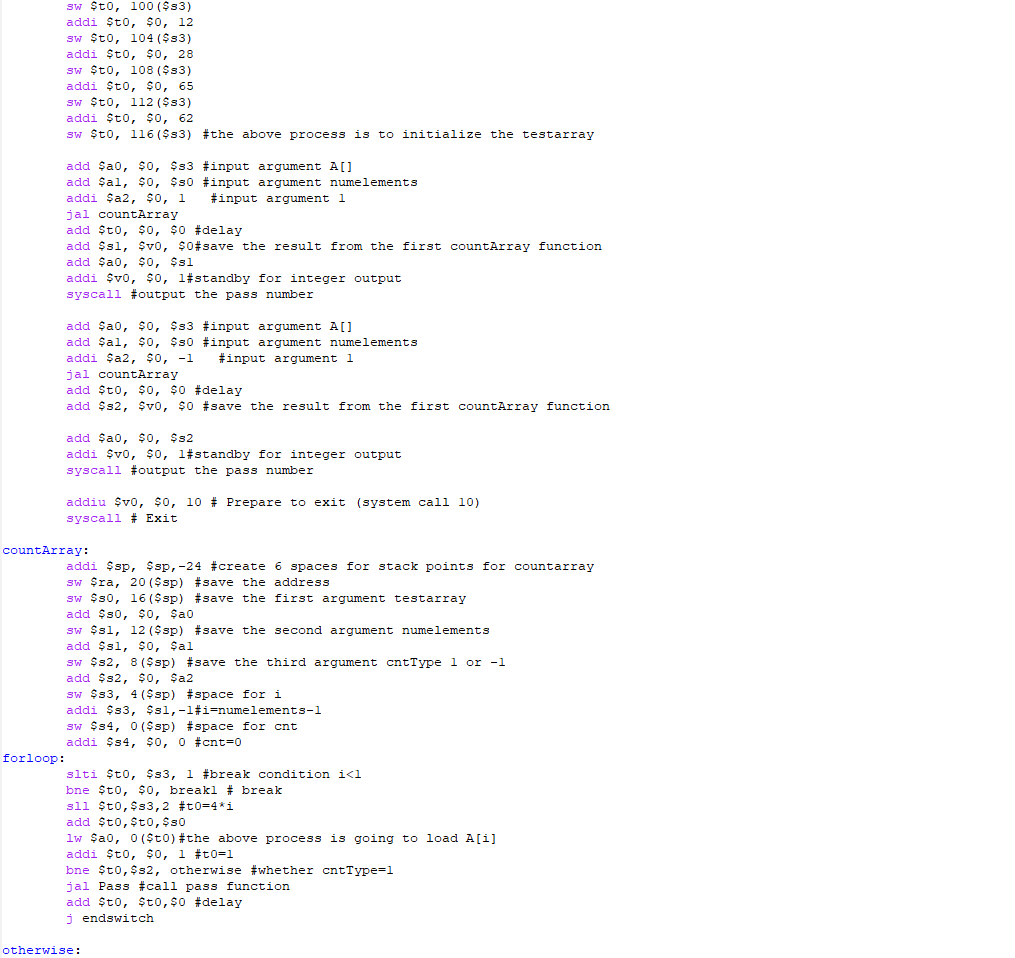
\includegraphics[scale=0.6]{mips2.png}
\end{figure}
\begin{figure}[H]
\centering
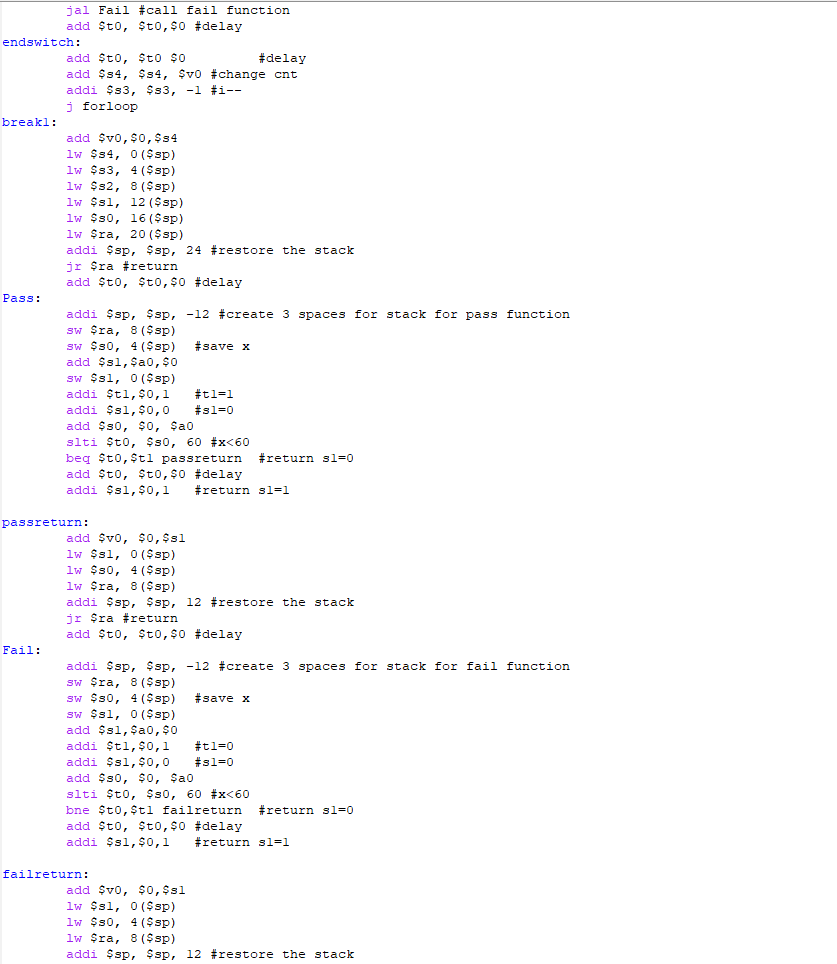
\includegraphics[scale=0.6]{mips3.png}
\end{figure}
\begin{figure}[H]
\centering
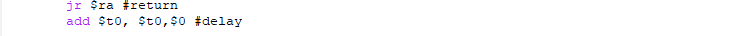
\includegraphics[scale=0.6]{mips4.png}
\end{figure}
\end{document}